\documentclass[12pt]{amsart}
\usepackage{nopageno}
\usepackage{amssymb, comment, float, latexsym, amsmath, amsthm, amscd, array, framed, graphicx, bigints, enumerate, mathtools, xcolor}
\usepackage{tikz}
\usetikzlibrary{matrix,arrows,calc}
\usetikzlibrary{positioning}
\usepackage{parskip}
\usepackage{caption} 
\usepackage{subcaption} 
\usepackage{multicol}
\usepackage[margin=2cm]{geometry}
\usepackage{hyperref}
\hypersetup{
    colorlinks=true,
    linkcolor=blue,
    filecolor=magenta,      
    urlcolor=cyan,
    pdftitle={Overleaf Example},
    %pdfpagemode=FullScreen,
    }

\newtheorem{thm}{Theorem}
\newtheorem{lem}[thm]{Lemma}
\newtheorem{prop}[thm]{Proposition}
\newtheorem{cor}[thm]{Corollary}
\newtheorem*{defin}{Definition}
\newtheorem*{ex}{Example}
\newtheorem*{exs}{Examples}
\newtheorem*{remark}{Remark}

\newcounter{mycounter}

\def\C{{\mathbb C}}
\def\Z{{\mathbb Z}}
\def\Q{{\mathbb Q}}
\def\R{{\mathbb R}}
\def\N{{\mathbb N}}
\def\F{{\mathbb F}}
\def\nCk{{^nC_k}}
\DeclareRobustCommand{\stirling}{\genfrac\{\}{0pt}{}}
\newcommand\nck[2]{\prescript{#1\mkern-2.5mu}{}C_{#2}}
\newcommand\nsk[2]{\prescript{#1\mkern-0.5mu}{}S_{#2}}

\renewcommand{\sectionname}{Worksheet}  

\begin{document}

\LARGE Dicey Exploration\\
\large A session for Sri Sri Ravishankar Vidya Mandir Students

\normalsize
Shantha Bhushan, Divakaran D, Tulsi Srinivasan\\
Azim Premji University

\rule{\textwidth}{0.1 cm}
\vspace{0.25cm}

\begin{enumerate}[1.]
    \item The standard dice has a cubical shape.  However, there are dice of other shapes.  We give images of three dice below\footnote{In a tetrahedral dice, the outcome is the number at the apex - as there is no top face.}.  What is common among all these shapes?
    \begin{figure}[ht]
        \centering
        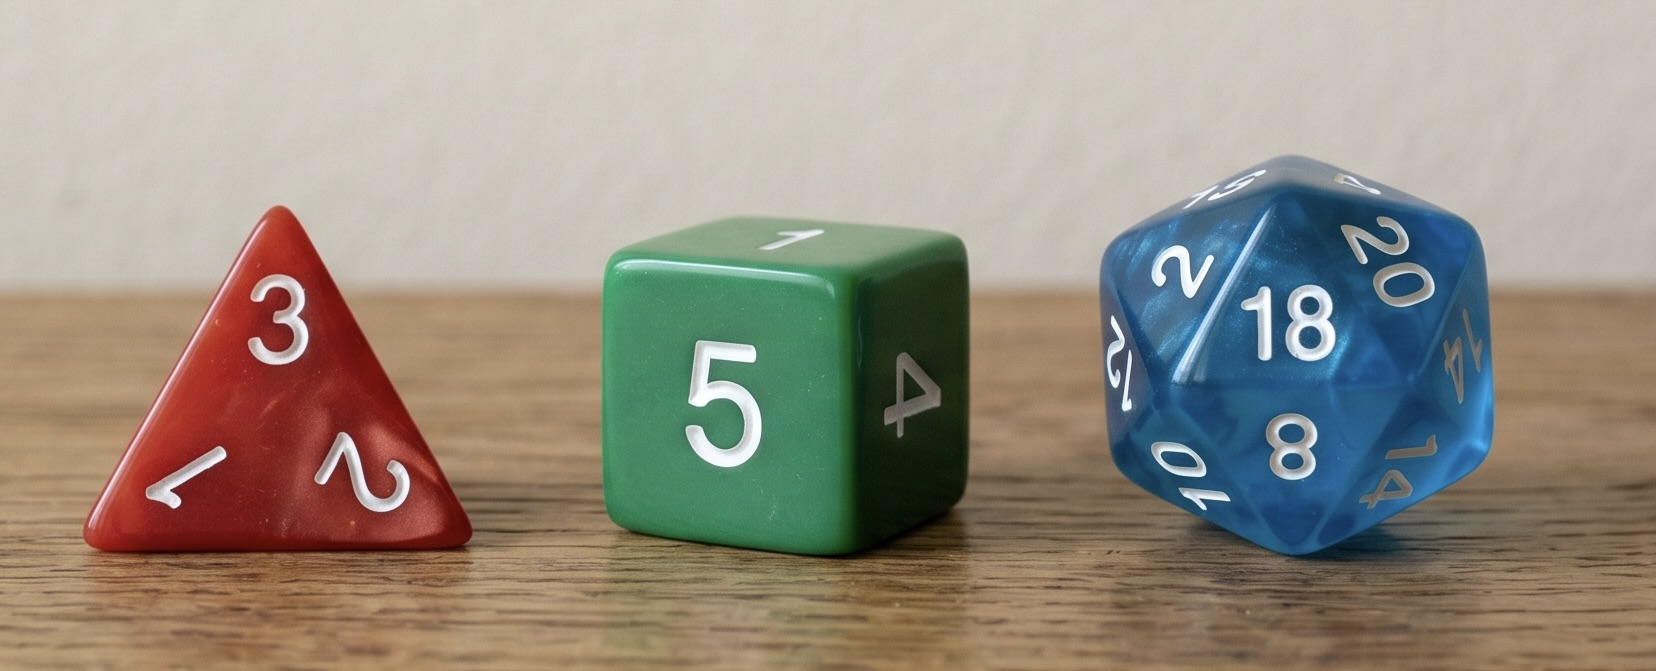
\includegraphics[width=0.5\linewidth]{Dice.jpeg}
    \end{figure}
    \item Construct your own dice.  Are all the numbers equally likely?  Give at least one example of a dice where all numbers are not equally likely.
    \item Consider a triangular prism as shown below.  Assume that the sides of the triangle are of unit length.  Show that if you choose height carefully, you can ensure that all sides are equally likely.  Are the surface areas of the sides equal when all sides are equally likely?
    \begin{figure}[ht]
        \centering
        \includegraphics[width=0.3\linewidth]{triangularprism.png}
    \end{figure}
    \item Are all sides equally likely for the dice given below?
    \begin{figure}[ht]
        \centering
        \includegraphics[width=0.3\linewidth]{cuboctahedron.png}
    \end{figure}
    \item Notice that all faces of the above dice didn't have the same shape.  This distinguishes the above dice from the dice in the first figure.  But, the faces are still regular (equilateral triangle and square), unlike the triangular prism.  Can you construct other shapes like that?  Are all sides equally likely?  

\end{enumerate}

\end{document}
\newpage

\LARGE Session for students of Ravishankar School

\normalsize
Shantha Bhushan, Divakaran D, Tulsi Srinivasan\\
Azim Premji University

\rule{\textwidth}{0.1 cm}

\section{Folding Tetrahedron}
\vspace{0.25cm}
\begin{enumerate}[1.]
   
\item Take a square sheet of paper.  Name the corners $A$, $B$, $C$, and $D$ as shown in the figure to the right.  Then fold side $AB$ on to $BC$ to get the fold $DB$.  Next fold $AB$ onto $CD$ to get the fold $MN$.  Finally, fold along $AN$ - let $AN$ and $DB$ intersect at $O$.  Can you find $\angle ANB$?  Assuming $D$ is the origin, can you find the coordinates of $O$ (in terms of the side of the square)?

\begin{figure}[h]
     \begin{subfigure}[b]{0.4\textwidth}
          \centering
          \resizebox{\linewidth}{!}{
            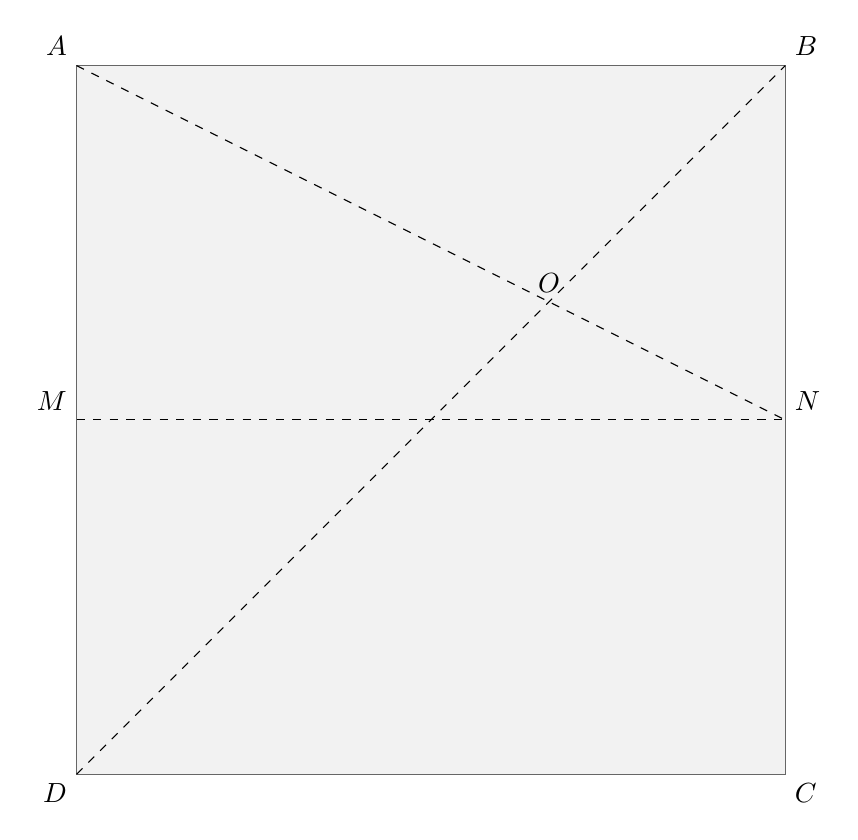
\begin{tikzpicture}
                \filldraw[color=black!60, fill=black!5](0,0) rectangle (9,9);
                \draw[dashed] (0,0) -- (9,9) node {};
                \draw[dashed] (0,4.5) -- (9,4.5) node {};
                \draw[dashed] (0,9) -- (9,4.5) node {};
                \draw (0,0) node[anchor=north east] {$D$};
                \draw (9,0) node[anchor=north west] {$C$};
                \draw (9,9) node[anchor= south west] {$B$};
                \draw (0,9) node[anchor=south east] {$A$};
                \draw (0,4.5) node[anchor=south east] {$M$};
                \draw (9,4.5) node[anchor=south west] {$N$};
                \draw (6,6) node[anchor=south] {$O$};
            \end{tikzpicture}}
     \end{subfigure}
     \begin{subfigure}[b]{0.4\textwidth}
          \centering
          \resizebox{\linewidth}{!}{
          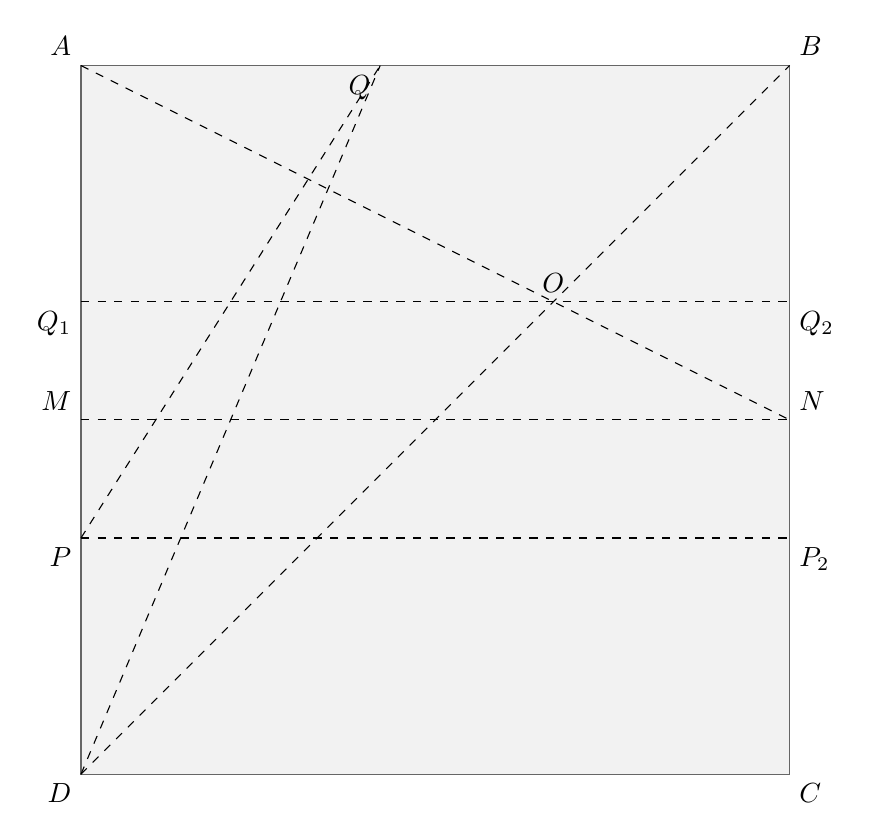
\begin{tikzpicture}
                \filldraw[color=black!60, fill=black!5](0,0) rectangle (9,9);
                \draw[dashed] (0,0) -- (9,9) node {};
                \draw[dashed] (0,4.5) -- (9,4.5) node {};
                \draw[dashed] (0,9) -- (9,4.5) node {};
                \draw (0,0) node[anchor=north east] {$D$};
                \draw (9,0) node[anchor=north west] {$C$};
                \draw (9,9) node[anchor= south west] {$B$};
                \draw (0,9) node[anchor=south east] {$A$};
                \draw (0,4.5) node[anchor=south east] {$M$};
                \draw (9,4.5) node[anchor=south west] {$N$};
                \draw (6,6) node[anchor=south] {$O$};
                \draw[dashed] (0,3) -- (9,3) node {};
                \draw (0,3) node[anchor=north east] {$P$};
                \draw (9,3) node[anchor=north west] {$P_2$};
                \draw[dashed] (0,6) -- (9,6) node {};
                \draw (0,6) node[anchor=north east] {$Q_1$};
                \draw (9,6) node[anchor=north west] {$Q_2$};
                \draw[dashed] (0,0) -- (3.8,9) node {};
                \draw (3.8,9) node[anchor=north east] {$Q$};
                \draw[dashed] (0,3) -- (3.8,9) node {};
            \end{tikzpicture}}
     \end{subfigure}
 \end{figure}
\item Fold $DC$ onto $O$ to obtain $PP_2$.  Fold $AB$ onto $PP_2$ to obtain $Q_1Q_2$.  Fold $AD$ onto $BD$, bisecting $\angle ADB$ - constructing the dashed line $DQ$.  Fold a line through $PQ$.  What is $\angle PQA$?
%\item Keeping $BC$ vertical, fold $BC$ onto $Q$, obtaining the dashed line $Q_3Q_4$.  
\item Construct $R$ on $DC$ such that $\angle APQ = \angle DPR$.
\begin{figure}[h]
     \begin{subfigure}[b]{0.4\textwidth}
          \centering
          \resizebox{\linewidth}{!}{
            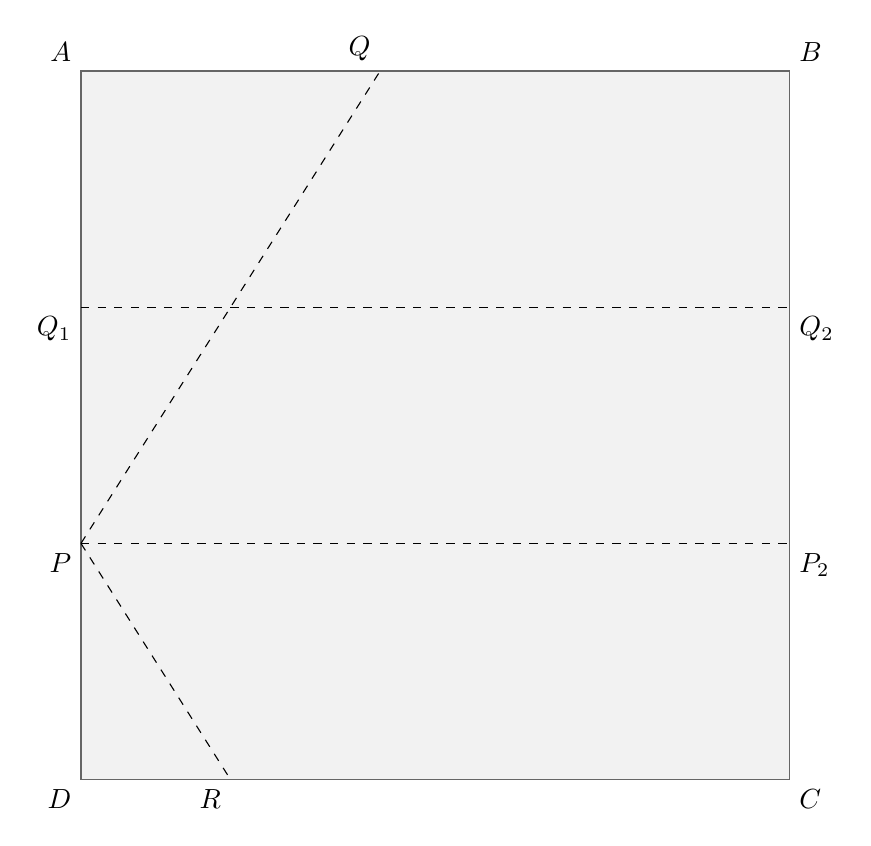
\begin{tikzpicture}
                \filldraw[color=black!60, fill=black!5](0,0) rectangle (9,9);
                %\draw[dashed] (0,0) -- (9,9) node {};
                %\draw[dashed] (0,4.5) -- (9,4.5) node {};
                %\draw[dashed] (0,9) -- (9,4.5) node {};
                \draw (0,0) node[anchor=north east] {$D$};
                \draw (9,0) node[anchor=north west] {$C$};
                \draw (9,9) node[anchor= south west] {$B$};
                \draw (0,9) node[anchor=south east] {$A$};
                %\draw (0,4.5) node[anchor=south east] {$M$};
                %\draw (9,4.5) node[anchor=south west] {$N$};
                %\draw (6,6) node[anchor=south] {$O$};
                \draw[dashed] (0,3) -- (9,3) node {};
                \draw (0,3) node[anchor=north east] {$P$};
                \draw (9,3) node[anchor=north west] {$P_2$};
                \draw[dashed] (0,6) -- (9,6) node {};
                \draw (0,6) node[anchor=north east] {$Q_1$};
                \draw (9,6) node[anchor=north west] {$Q_2$};
                %\draw[dashed] (0,0) -- (3.8,9) node {};
                \draw (3.8,9) node[anchor=south east] {$Q$};
                \draw[dashed] (0,3) -- (3.8,9) node {};
                %\draw[dashed] (6.4,0) -- (6.4,9) node {};
                %\draw (6.4,0) node[anchor=south east] {$Q_3$};
                %\draw (6.4,9) node[anchor=north east] {$Q_4$};
                \draw[dashed] (0,3) -- (1.9,0) node {};
                \draw (1.9,0) node[anchor=north east] {$R$};
            
            \end{tikzpicture}}
     \end{subfigure}
     \begin{subfigure}[b]{0.4\textwidth}
          \centering
          \resizebox{\linewidth}{!}{
          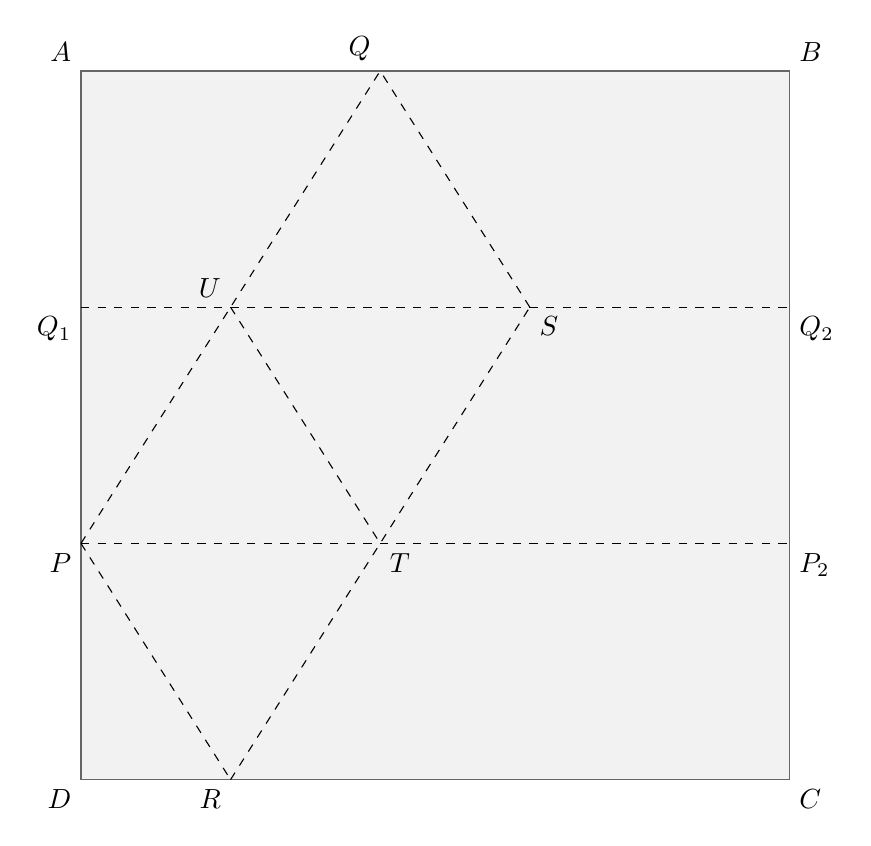
\begin{tikzpicture}
                \filldraw[color=black!60, fill=black!5](0,0) rectangle (9,9);
                %\draw[dashed] (0,0) -- (9,9) node {};
                %\draw[dashed] (0,4.5) -- (9,4.5) node {};
                %\draw[dashed] (0,9) -- (9,4.5) node {};
                \draw (0,0) node[anchor=north east] {$D$};
                \draw (9,0) node[anchor=north west] {$C$};
                \draw (9,9) node[anchor= south west] {$B$};
                \draw (0,9) node[anchor=south east] {$A$};
                %\draw (0,4.5) node[anchor=south east] {$M$};
                %\draw (9,4.5) node[anchor=south west] {$N$};
                %\draw (6,6) node[anchor=south] {$O$};
                \draw[dashed] (0,3) -- (9,3) node {};
                \draw (0,3) node[anchor=north east] {$P$};
                \draw (9,3) node[anchor=north west] {$P_2$};
                \draw[dashed] (0,6) -- (9,6) node {};
                \draw (0,6) node[anchor=north east] {$Q_1$};
                \draw (9,6) node[anchor=north west] {$Q_2$};
                %\draw[dashed] (0,0) -- (3.8,9) node {};
                \draw (3.8,9) node[anchor=south east] {$Q$};
                \draw[dashed] (0,3) -- (3.8,9) node {};
                %\draw[dashed] (6.4,0) -- (6.4,9) node {};
                %\draw (6.4,0) node[anchor=south east] {$Q_3$};
                %\draw (6.4,9) node[anchor=north east] {$Q_4$};
                \draw[dashed] (0,3) -- (1.9,0) node {};
                \draw (1.9,0) node[anchor=north east] {$R$};
                \draw[dashed] (1.9,0) -- (5.7,6) node {};
                \draw (5.7,6) node[anchor=north west] {$S$};
                \draw[dashed] (5.7,6) -- (3.8,9) node {};
                \draw (1.9,6) node[anchor=south east] {$U$};
                \draw (3.8,3) node[anchor=north west] {$T$};
                \draw[dashed] (1.9,6) -- (3.8,3) node {};
            \end{tikzpicture}}
     \end{subfigure}
 \end{figure}
 \item Bisect $\angle PRC$ to obtain $RS$.  Let the intersection of $RS$ and $PP_2$ be $T$.  Let the intersection of $PQ$ and $Q_1Q_3$ be $U$.  Fold through $UT$.  The four triangles $PRT$, $PTU$, $TUS$, and $USQ$ form the net of the tetrahedron.  Use the existing creases to form the tetrahedron.
 
\end{enumerate}




